%---------------
%╔═╗╔═╗╔╦╗╦ ╦╔═╗
%╚═╗║╣  ║ ║ ║╠═╝
%╚═╝╚═╝ ╩ ╚═╝╩  
%---------------
\documentclass[12pt,oneside,a4paper]{report}

% DOCUMENT SETUP
\usepackage[left=3cm, 
			right=2.5cm, 
			top=2.5cm, 
			bottom=2.5cm, 
			includehead, 
			includefoot]{geometry}

% line spacing
\usepackage{setspace}
\setstretch{1,25} % 15/12 --> 1.25

%de­fines Adobe Times Ro­man as de­fault text font
\usepackage{mathptmx}
\usepackage{times} % needed for acronym package

%PDF linking package
\usepackage[hidelinks]{hyperref}

% Language Setup
\usepackage[ngerman]{babel}
% language specific bibliography style
\usepackage[numbers]{natbib}
\usepackage[fixlanguage]{babelbib}
\selectbiblanguage{german}
% bliographystyle setup
% default style names: apalike alphadin ieeetr IEEEtranSN apalike2 alphadin 
% babel specific: babplain, babplai3, babalpha, babunsrt, bababbrv, bababbr3 unsrt 
\bibliographystyle{unsrturl}

% encoding setup
% T1 font encoding for languages that use a latin alphabet
\usepackage[T1]{fontenc} 

% enhanced input encoding handling - utf8 for äÄüÜöÖß...
\usepackage[utf8]{inputenc}
%\usepackage{ucs}%utf8x suppart

% after babel - set chapter string
\AtBeginDocument{\renewcommand{\chaptername}{}}

% enumeration
\usepackage{enumitem}
% tabular extension tabularx
\usepackage{tabularx}

% math packages
\usepackage{amsmath}
\usepackage{nicefrac}
\usepackage{amsthm}
\usepackage{amsbsy}
\usepackage{amssymb}
\usepackage{amsfonts}
\usepackage{MnSymbol}

% patches for latex
\usepackage{fixltx2e}

%special characters
\usepackage{amssymb}
\usepackage{upgreek,textgreek}

% acronym package
\usepackage[printonlyused, footnote]{acronym}

% breakable text in \seqsplit{}
\usepackage{seqsplit}

% \textmu
\usepackage{textcomp}

% package provides a way to compile sections of a document using the same preamble as the main document
\usepackage{subfiles}

% driver-independent color extension - used by listings,tabularx
\usepackage[usenames,dvipsnames,table,xcdraw]{xcolor}

% -- SYNTAX HIGHLIGHTING --
\usepackage{listings}
%% bash command line Syntax Highlighting
\lstdefinestyle{BASH_CMD}{ 
  columns=fullflexible,            % copy pasteable listings
  language=bash,
  basicstyle=\small\sffamily,
  basicstyle   = \small \ttfamily,
  keywordstyle = [1]\small \ttfamily,
  keywordstyle = [2]\small \ttfamily,
  commentstyle = \small \ttfamily,
  numbers=none,
  captionpos=b, 
  breaklines=true,
  numberstyle=\tiny,
  numbersep=3pt,
  frame=tlrb,
  columns=fullflexible,
  backgroundcolor=\color{white!20},
  linewidth=\linewidth,
  literate=                        % replace in code
     {Ö}{{\"O}}1
     {Ä}{{\"A}}1
     {Ü}{{\"U}}1
     {ß}{{\ss}}2
     {ü}{{\"u}}1
     {ä}{{\"a}}1
     {ö}{{\"o}}1
}
 % adds style BASH_CMD
%% Matlab Syntax Highlighting
\colorlet{keyword}{blue!100!black!80}
\colorlet{STD}{Lavender}
\colorlet{comment}{green!90!black!90}
\definecolor{mygreen}{rgb}{0,0.6,0}
\definecolor{mygray}{rgb}{0.5,0.5,0.5}
\definecolor{mymauve}{rgb}{0.58,0,0.82}


\lstdefinestyle{BASH_SCRIPT}{ 
  language     = bash,
  basicstyle   = \footnotesize \ttfamily,
  keywordstyle = [1]\color{keyword}\bfseries,
  keywordstyle = [2]\color{STD}\bfseries,
  commentstyle = \color{mygreen}\itshape,
  backgroundcolor=\color{white},   % choose the background color; you must add \usepackage{color} 
  columns=fullflexible,            % copy pasteable listings
                                   % or \usepackage{xcolor}
  basicstyle=\footnotesize,        % the size of the fonts that are used for the code
  breakatwhitespace=false,         % sets if automatic breaks should only happen at whitespace
  breaklines=true,                 % sets automatic line breaking
  captionpos=b,                    % sets the caption-position to bottom
  extendedchars=true,              % lets you use non-ASCII characters; for 8-bits encodings only,
                                   % does not work with UTF-8
  frame=single,                    % adds a frame around the code
  keepspaces=true,                 % keeps spaces in text, useful for keeping indentation of code
                                   % (possibly needs columns=flexible)
  numbers=left,                    % where to put the line-numbers; possible values are 
                                   % (none, left, right)
  numbersep=5pt,                   % how far the line-numbers are from the code
  numberstyle=\tiny\color{mygray}, % the style that is used for the line-numbers
  rulecolor=\color{black},         % if not set, the frame-color may be changed on line-breaks
                                   % within not-black text (e.g. comments (green here))
  showspaces=false,                % show spaces everywhere adding particular underscores; it
  	                               % overrides 'showstringspaces'
  showstringspaces=false,          % underline spaces within strings only
  showtabs=false,                  % show tabs within strings adding particular underscores
  stepnumber=1,                    % the step between two line-numbers. If it's 1, each line 
                                   % will be numbered
  stringstyle=\color{mymauve},     % string literal style
  tabsize=2,                       % sets default tabsize to 2 spaces
  title=\lstname,                  % set title name
  literate=                        % replace in code
     {Ö}{{\"O}}1
     {Ä}{{\"A}}1
     {Ü}{{\"U}}1
     {ß}{{\ss}}2
     {ü}{{\"u}}1
     {ä}{{\"a}}1
     {ö}{{\"o}}1
} % adds style BASH_SCRIPT
% Matlab Syntax Highlighting
\colorlet{keyword}{blue!100!black!80}
\colorlet{STD}{red}
\colorlet{comment}{green!90!black!90}
\definecolor{mygreen}{rgb}{0,0.6,0}
\definecolor{mygray}{rgb}{0.5,0.5,0.5}
\definecolor{mymauve}{rgb}{0.58,0,0.82}


\lstdefinestyle{LATEX}{ 
  language     = [LaTeX]{TeX},
  basicstyle   = \footnotesize \ttfamily,
  keywordstyle = [1]\color{keyword}\bfseries,
  keywordstyle = [2]\color{comment}\bfseries,
  commentstyle = \color{mygray}\itshape,
  %backgroundcolor=\color{white},   % choose the background color; you must add \usepackage{color} 
                                   % or \usepackage{xcolor}
  basicstyle=\footnotesize,        		   % the size of the fonts that are used for the code
  breakatwhitespace=false,         % sets if automatic breaks should only happen at whitespace
  columns=fullflexible,            % copy pasteable listings
  breaklines=true,                 % sets automatic line breaking
  captionpos=c,                    % sets the caption-position to bottom
  extendedchars=true,              % lets you use non-ASCII characters; for 8-bits encodings only,
                                   % does not work with UTF-8
  frame=single,                    % adds a frame around the code
  keepspaces=true,                 % keeps spaces in text, useful for keeping indentation of code
                                   % (possibly needs columns=flexible)
  numbers=left,                    % where to put the line-numbers; possible values are 
                                   % (none, left, right)
  numbersep=4pt,                   % how far the line-numbers are from the code
  numberstyle=\tiny\color{mygray}, % the style that is used for the line-numbers
  rulecolor=\color{black},         % if not set, the frame-color may be changed on line-breaks
                                   % within not-black text (e.g. comments (green here))
  showspaces=false,                % show spaces everywhere adding particular underscores; it
  	                               % overrides 'showstringspaces'
  showstringspaces=false,          % underline spaces within strings only
  showtabs=false,                  % show tabs within strings adding particular underscores
  stepnumber=1,                    % the step between two line-numbers. If it's 1, each line 
                                   % will be numbered
  stringstyle=\color{mymauve},     % string literal style
  tabsize=2,                       % sets default tabsize to 2 spaces
  title=\lstname,                  % set title name
  literate=                        % replace in code
     {Ö}{{\"O}}1
     {Ä}{{\"A}}1
     {Ü}{{\"U}}1
     {ß}{{\ss}}2
     {ü}{{\"u}}1
     {ä}{{\"a}}1
     {ö}{{\"o}}1
} % adds style LATEX
%% Matlab Syntax Highlighting
\colorlet{keyword}{blue!100!black!80}
\colorlet{STD}{Lavender}
\colorlet{comment}{green!90!black!90}
\definecolor{mygreen}{rgb}{0,0.6,0}
\definecolor{mygray}{rgb}{0.5,0.5,0.5}
\definecolor{mymauve}{rgb}{0.58,0,0.82}


\lstdefinestyle{MATLAB}{ 
  language     = Matlab,
  basicstyle   = \footnotesize \ttfamily,
  keywordstyle = [1]\color{keyword}\bfseries,
  keywordstyle = [2]\color{STD}\bfseries,
  commentstyle = \color{mygreen}\itshape,
  backgroundcolor=\color{white},   % choose the background color; you must add \usepackage{color} 
                                   % or \usepackage{xcolor}
  basicstyle=\footnotesize,        % the size of the fonts that are used for the code
  breakatwhitespace=false,         % sets if automatic breaks should only happen at whitespace
  columns=fullflexible,            % copy pasteable listings
  breaklines=false,                % sets automatic line breaking
  captionpos=c,                    % sets the caption-position to bottom
  extendedchars=true,              % lets you use non-ASCII characters; for 8-bits encodings only,
                                   % does not work with UTF-8
  frame=single,                    % adds a frame around the code
  keepspaces=true,                 % keeps spaces in text, useful for keeping indentation of code
                                   % (possibly needs columns=flexible)
  numbers=left,                    % where to put the line-numbers; possible values are 
                                   % (none, left, right)
  numbersep=5pt,                   % how far the line-numbers are from the code
  numberstyle=\tiny\color{mygray}, % the style that is used for the line-numbers
  rulecolor=\color{black},         % if not set, the frame-color may be changed on line-breaks
                                   % within not-black text (e.g. comments (green here))
  showspaces=false,                % show spaces everywhere adding particular underscores; it
  	                               % overrides 'showstringspaces'
  showstringspaces=false,          % underline spaces within strings only
  showtabs=false,                  % show tabs within strings adding particular underscores
  stepnumber=1,                    % the step between two line-numbers. If it's 1, each line 
                                   % will be numbered
  stringstyle=\color{mymauve},     % string literal style
  tabsize=2,                       % sets default tabsize to 2 spaces
  title=\lstname,                  % set title name
  literate=                        % replace in code
     {Ö}{{\"O}}1
     {Ä}{{\"A}}1
     {Ü}{{\"U}}1
     {ß}{{\ss}}2
     {ü}{{\"u}}1
     {ä}{{\"a}}1
     {ö}{{\"o}}1
} % adds style MATLAB
% Matlab Syntax Highlighting
\colorlet{keyword}{blue!100!black!80}
\colorlet{STD}{Lavender}
\colorlet{comment}{green!90!black!90}
\definecolor{mygreen}{rgb}{0,0.6,0}
\definecolor{mygray}{rgb}{0.5,0.5,0.5}
\definecolor{mymauve}{rgb}{0.58,0,0.82}


\lstdefinestyle{PYTHON}{ 
  language     = Python,
  basicstyle   = \footnotesize \ttfamily,
  keywordstyle = [1]\color{keyword}\bfseries,
  keywordstyle = [2]\color{STD}\bfseries,
  commentstyle = \color{mygreen}\itshape,
  backgroundcolor=\color{white},   % choose the background color; you must add \usepackage{color} 
                                   % or \usepackage{xcolor}
  basicstyle=\footnotesize,        % the size of the fonts that are used for the code
  columns=fullflexible,            % copy pasteable listings
  breakatwhitespace=false,         % sets if automatic breaks should only happen at whitespace
  breaklines=false,                % sets automatic line breaking
  captionpos=c,                    % sets the caption-position to bottom
  extendedchars=true,              % lets you use non-ASCII characters; for 8-bits encodings only,
                                   % does not work with UTF-8
  frame=single,                    % adds a frame around the code
  keepspaces=true,                 % keeps spaces in text, useful for keeping indentation of code
                                   % (possibly needs columns=flexible)
  numbers=left,                    % where to put the line-numbers; possible values are 
                                   % (none, left, right)
  numbersep=5pt,                   % how far the line-numbers are from the code
  numberstyle=\tiny\color{mygray}, % the style that is used for the line-numbers
  rulecolor=\color{black},         % if not set, the frame-color may be changed on line-breaks
                                   % within not-black text (e.g. comments (green here))
  showspaces=false,                % show spaces everywhere adding particular underscores; it
  	                               % overrides 'showstringspaces'
  showstringspaces=false,          % underline spaces within strings only
  showtabs=false,                  % show tabs within strings adding particular underscores
  stepnumber=1,                    % the step between two line-numbers. If it's 1, each line 
                                   % will be numbered
  stringstyle=\color{mymauve},     % string literal style
  tabsize=2,                       % sets default tabsize to 2 spaces
  title=\lstname,                  % set title name
  literate=                        % replace in code
     {Ö}{{\"O}}1
     {Ä}{{\"A}}1
     {Ü}{{\"U}}1
     {ß}{{\ss}}2
     {ü}{{\"u}}1
     {ä}{{\"a}}1
     {ö}{{\"o}}1
} % adds style PYTHON
%% Matlab Syntax Highlighting
\colorlet{keyword}{blue!100!black!80}
\colorlet{STD}{Lavender}
\colorlet{comment}{green!90!black!90}
\definecolor{mygreen}{rgb}{0,0.6,0}
\definecolor{mygray}{rgb}{0.5,0.5,0.5}
\definecolor{mymauve}{rgb}{0.58,0,0.82}


\lstdefinestyle{CPP}{ 
  language     = C++,
  basicstyle   = \footnotesize \ttfamily,
  keywordstyle = [1]\color{keyword}\bfseries,
  keywordstyle = [2]\color{STD}\bfseries,
  commentstyle = \color{mygreen}\itshape,
  backgroundcolor=\color{white},   % choose the background color; you must add \usepackage{color} 
                                   % or \usepackage{xcolor}
  columns=fullflexible,            % copy pasteable listings
  basicstyle=\footnotesize,        % the size of the fonts that are used for the code
  breakatwhitespace=false,         % sets if automatic breaks should only happen at whitespace
  breaklines=false,                % sets automatic line breaking
  captionpos=c,                    % sets the caption-position to bottom
  extendedchars=true,              % lets you use non-ASCII characters; for 8-bits encodings only,
                                   % does not work with UTF-8
  frame=single,                    % adds a frame around the code
  keepspaces=true,                 % keeps spaces in text, useful for keeping indentation of code
                                   % (possibly needs columns=flexible)
  numbers=left,                    % where to put the line-numbers; possible values are 
                                   % (none, left, right)
  numbersep=5pt,                   % how far the line-numbers are from the code
  numberstyle=\tiny\color{mygray}, % the style that is used for the line-numbers
  rulecolor=\color{black},         % if not set, the frame-color may be changed on line-breaks
                                   % within not-black text (e.g. comments (green here))
  showspaces=false,                % show spaces everywhere adding particular underscores; it
  	                               % overrides 'showstringspaces'
  showstringspaces=false,          % underline spaces within strings only
  showtabs=false,                  % show tabs within strings adding particular underscores
  stepnumber=1,                    % the step between two line-numbers. If it's 1, each line 
                                   % will be numbered
  stringstyle=\color{mymauve},     % string literal style
  tabsize=2,                       % sets default tabsize to 2 spaces
  title=\lstname,                  % set title name
  literate=                        % replace in code
     {Ö}{{\"O}}1
     {Ä}{{\"A}}1
     {Ü}{{\"U}}1
     {ß}{{\ss}}2
     {ü}{{\"u}}1
     {ä}{{\"a}}1
     {ö}{{\"o}}1
} % adds style CPP
%% Matlab Syntax Highlighting
\colorlet{keyword}{blue!100!black!80}
\colorlet{STD}{Lavender}
\colorlet{comment}{green!90!black!90}
\definecolor{mygreen}{rgb}{0,0.6,0}
\definecolor{mygray}{rgb}{0.5,0.5,0.5}
\definecolor{mymauve}{rgb}{0.58,0,0.82}


\lstdefinestyle{C}{ 
  language     = C,
  basicstyle   = \footnotesize \ttfamily,
  keywordstyle = [1]\color{keyword}\bfseries,
  keywordstyle = [2]\color{STD}\bfseries,
  commentstyle = \color{mygreen}\itshape,
  backgroundcolor=\color{white},   % choose the background color; you must add \usepackage{color} 
  columns=fullflexible,            % copy pasteable listings
                                   % or \usepackage{xcolor}
  basicstyle=\footnotesize,        % the size of the fonts that are used for the code
  breakatwhitespace=false,         % sets if automatic breaks should only happen at whitespace
  breaklines=false,                % sets automatic line breaking
  captionpos=c,                    % sets the caption-position to bottom
  extendedchars=true,              % lets you use non-ASCII characters; for 8-bits encodings only,
                                   % does not work with UTF-8
  frame=single,                    % adds a frame around the code
  keepspaces=true,                 % keeps spaces in text, useful for keeping indentation of code
                                   % (possibly needs columns=flexible)
  numbers=left,                    % where to put the line-numbers; possible values are 
                                   % (none, left, right)
  numbersep=5pt,                   % how far the line-numbers are from the code
  numberstyle=\tiny\color{mygray}, % the style that is used for the line-numbers
  rulecolor=\color{black},         % if not set, the frame-color may be changed on line-breaks
                                   % within not-black text (e.g. comments (green here))
  showspaces=false,                % show spaces everywhere adding particular underscores; it
  	                               % overrides 'showstringspaces'
  showstringspaces=false,          % underline spaces within strings only
  showtabs=false,                  % show tabs within strings adding particular underscores
  stepnumber=1,                    % the step between two line-numbers. If it's 1, each line 
                                   % will be numbered
  stringstyle=\color{mymauve},     % string literal style
  tabsize=2,                       % sets default tabsize to 2 spaces
  title=\lstname,                  % set title name
  literate=                        % replace in code
     {Ö}{{\"O}}1
     {Ä}{{\"A}}1
     {Ü}{{\"U}}1
     {ß}{{\ss}}2
     {ü}{{\"u}}1
     {ä}{{\"a}}1
     {ö}{{\"o}}1
} % adds style C
%% JSON Syntax Highlighting
\colorlet{keyword}{blue!100!black!80}
\colorlet{STD}{Lavender}
\colorlet{comment}{green!90!black!90}
\definecolor{mygreen}{rgb}{0,0.6,0}
\definecolor{mygray}{rgb}{0.5,0.5,0.5}
\definecolor{mymauve}{rgb}{0.58,0,0.82}

\newcommand\JSONnumbervaluestyle{\color{blue}}
\newcommand\JSONstringvaluestyle{\color{red}}

\newif\ifcolonfoundonthisline

\makeatletter

\lstdefinelanguage{json}
{
  showstringspaces    = false,
  keywords            = {false,true},
  alsoletter          = 0123456789.,
  morestring          = [s]{"}{"},
  morestring          = [s]{'}{'},
  stringstyle         = \ifcolonfoundonthisline\JSONstringvaluestyle\fi,
  MoreSelectCharTable =%
    \lst@DefSaveDef{`:}\colon@json{\processColon@json},
  basicstyle          = \ttfamily,
  keywordstyle        = \ttfamily\bfseries,
}

% flip the switch if a colon is found in Pmode
\newcommand\processColon@json{
  \colon@json%
  \ifnum\lst@mode=\lst@Pmode%
    \global\colonfoundonthislinetrue%
  \fi
}

\lst@AddToHook{Output}{%
  \ifcolonfoundonthisline%
    \ifnum\lst@mode=\lst@Pmode%
      \def\lst@thestyle{\JSONnumbervaluestyle}%
    \fi
  \fi
  %override by keyword style if a keyword is detected!
  \lsthk@DetectKeywords% 
}

% reset the switch at the end of line
\lst@AddToHook{EOL}%
  {\global\colonfoundonthislinefalse}

\makeatother



\lstdefinestyle{JSON}{ 
  language     = json,
  basicstyle   = \footnotesize \ttfamily,
  keywordstyle = [1]\color{keyword}\bfseries,
  keywordstyle = [2]\color{STD}\bfseries,
  commentstyle = \color{mygreen}\itshape,
  backgroundcolor=\color{white},   % choose the background color; you must add \usepackage{color} 
                                   % or \usepackage{xcolor}
  basicstyle=\footnotesize,        % the size of the fonts that are used for the code
  columns=fullflexible,            % copy pasteable listings
  breakatwhitespace=false,         % sets if automatic breaks should only happen at whitespace
  breaklines=false,                % sets automatic line breaking
  captionpos=c,                    % sets the caption-position to bottom
  extendedchars=true,              % lets you use non-ASCII characters; for 8-bits encodings only,
                                   % does not work with UTF-8
  frame=single,                    % adds a frame around the code
  keepspaces=true,                 % keeps spaces in text, useful for keeping indentation of code
                                   % (possibly needs columns=flexible)
  numbers=left,                    % where to put the line-numbers; possible values are 
                                   % (none, left, right)
  numbersep=5pt,                   % how far the line-numbers are from the code
  numberstyle=\tiny\color{mygray}, % the style that is used for the line-numbers
  rulecolor=\color{black},         % if not set, the frame-color may be changed on line-breaks
                                   % within not-black text (e.g. comments (green here))
  showspaces=false,                % show spaces everywhere adding particular underscores; it
  	                               % overrides 'showstringspaces'
  showstringspaces=false,          % underline spaces within strings only
  showtabs=false,                  % show tabs within strings adding particular underscores
  stepnumber=1,                    % the step between two line-numbers. If it's 1, each line 
                                   % will be numbered
  stringstyle=\color{mymauve},     % string literal style
  tabsize=2,                       % sets default tabsize to 2 spaces
  title=\lstname,                  % set title name
  literate=                        % replace in code
     {Ö}{{\"O}}1
     {Ä}{{\"A}}1
     {Ü}{{\"U}}1
     {ß}{{\ss}}2
     {ü}{{\"u}}1
     {ä}{{\"a}}1
     {ö}{{\"o}}1
} % adds style JSON

% HEADLINE CFG
\usepackage{fancyhdr} % Headers and footers
\usepackage{lastpage}
\usepackage{nopageno}
\setlength{\headheight}{1.5cm}
\pagestyle{fancy} % All pages have headers and footers
\fancyhead{} % Blank out the default header
\fancyfoot{} % Blank out the default footer
\fancyhead[L]{}
\fancyhead[C]{}
\fancyhead[R]{}
\fancyfoot[L]{}
\fancyfoot[C]{\thepage}
\fancyfoot[R]{}
% override plain page style for \part, \chapter or 
% \maketitle, which implicit specifies plain page style
\fancypagestyle{plain} 
{
	\fancyhead[L]{}
	\fancyhead[C]{}
	\fancyhead[R]{}
	\fancyfoot[L]{}
	\fancyfoot[C]{\thepage}
	\fancyfoot[R]{}
}
% set list pagestyle
\fancypagestyle{lists} 
{
	\fancyhead[L]{}
	\fancyhead[C]{}
	\fancyhead[R]{}
	\fancyfoot[L]{}
	\fancyfoot[C]{\thepage}
	\fancyfoot[R]{}
}

\renewcommand{\chaptermark}[1]{\markright{#1}{}}
\renewcommand{\sectionmark}[1]{\markright{#1}{}}
\renewcommand{\headrulewidth}{0pt}
\renewcommand{\footrulewidth}{0pt}

	
\usepackage{verbatim}
\usepackage{graphicx}
\usepackage{epstopdf}

% floating prevention packages
\usepackage{float}    % used with [H] positioning parameter
\usepackage{placeins} % \FloatBarrier 

% tikz packages
\usepackage{tikz}
\usepackage{caption}
\usepackage[list=true,listformat=simple]{subcaption}
\usepackage{standalone}
\usepackage{pgfplots}


% include only specified tex files - uncommend unneeded
\includeonly{preface/cover,
             preface/abstract,
             preface/tableofcontents,
             preface/listoffigures,
             preface/listoftables,
             preface/lstlistoflistings,
             appendix/bibliography}

%-------------------
%╔═╗╔╦╗╦═╗╦╔╗╔╔═╗╔═╗
%╚═╗ ║ ╠╦╝║║║║║ ╦╚═╗
%╚═╝ ╩ ╩╚═╩╝╚╝╚═╝╚═╝
%-------------------
\newcommand{\strLecture}{Signale, Systeme und Sensoren}
\newcommand{\strDate}{\today}
\newcommand{\strAuthorA}{J. Altmeyer}
\newcommand{\strAuthorB}{M. Kieser}
\newcommand{\strAuthorAEmail}{jualtmey@htwg-konstanz.de}
\newcommand{\strAuthorBEmail}{makieser@htwg-konstanz.de}
% Versuchsbeschreibung 
\newcommand{\strTopic}{Labor Signale, Systeme und Sensoren WS 2015/16}
\newcommand{\strAbstract}{TODO:Zusammenfassung etwa 100 Worte.}
% hyperref customization
\hypersetup{
	pdftitle    ={\strTopic}, % title
	pdfsubject	={\strLecture}, % subject of the document
	pdfauthor	={\strAuthorA, \strAuthorB}, % author
	pdfkeywords	={}, % list of keywords
	pdfcreator	={}, % creator of the document
	pdfproducer	={}, % producer of the document
	colorlinks=false, % false: boxed links; true: colored links
	linkcolor=red, % color of internal links (change box color with linkbordercolor)
    citecolor=green, % color of links to bibliography
    filecolor=magenta, % color of file links
    urlcolor=cyan, % color of external links
	%bookmarks=true, % show bookmarks bar?
	unicode=true, % non-Latin characters in Acrobat’s bookmarks
	pdftoolbar=true, % show Acrobat’s toolbar?
	pdfmenubar=true, % show Acrobat’s menu?
    pdffitwindow=false, % window fit to page when opened
	pdfnewwindow=true % links in new PDF window
}

%-----------------------------------------
% ╔╗ ╔═╗╔═╗╦╔╗╔  ╔╦╗╔═╗╔═╗╦ ╦╔╦╗╔═╗╔╗╔╔╦╗ 
% ╠╩╗║╣ ║ ╦║║║║   ║║║ ║║  ║ ║║║║║╣ ║║║ ║  
% ╚═╝╚═╝╚═╝╩╝╚╝  ═╩╝╚═╝╚═╝╚═╝╩ ╩╚═╝╝╚╝ ╩  
%-----------------------------------------

\begin{document}
\pagenumbering{Roman} 

%\setcounter{section}{0}

\begin{titlepage}

\vspace*{-3.5cm}

\begin{flushleft}
\hspace*{-1cm} 
\includegraphics[width=15.7cm]{preface/htwg-logo}
\end{flushleft}

\vspace{1cm}

\begin{center}
	\large{
		\textbf{\strLecture} \\[2cm]
	}
	\Huge{
		\textbf{\strTopic} \\[2cm]
	}
	\Large{
		\textbf{\strAuthorA, \strAuthorB}} \\[3cm]
	\large{
		\textbf{} \\[2.3cm]
	}
	
	\large{
		\textbf{Konstanz, \strDate}
	}
\end{center}

\end{titlepage}
\thispagestyle{empty}




\begin{center}
{\Large \textbf{Zusammenfassung (Abstract)}}
\end{center}

\bigskip

\begin{center}
	\begin{tabular}{p{2.8cm}p{5cm}p{5cm}}
		Thema: & \multicolumn{2}{p{10cm}}{\raggedright\strTopic} \\
		 & & \\
		Autoren: & \strAuthorA & \href{mailto:\strAuthorAEmail}{\strAuthorAEmail} \\
		 & \strAuthorB & \href{mailto:\strAuthorBEmail}{\strAuthorBEmail} \\
		 & & \\
		Betreuer: & Prof. Dr. Matthias O. Franz & \href{mailto:mfranz@htwg-konstanz.de}{mfranz@htwg-konstanz.de} \\
		 &  Jürgen Keppler & \href{mailto:juergen.keppler@htwg-konstanz.de}{juergen.keppler@htwg-konstanz.de} \\
		 &  Martin Miller & \href{mailto:martin.miller@htwg-konstanz.de}{martin.miller@htwg-konstanz.de} \\
	\end{tabular}
\end{center}

\bigskip

\noindent
\strAbstract

\thispagestyle{lists}



\clearpage

%
% TABLE OF CONTENTS
%
\thispagestyle{lists}
%
% TABLE OF CONTENTS
%
\tableofcontents
\thispagestyle{plain}
\newpage

%
% Abbildungsverzeichnis
%
%
% Abbildungsverzeichnis
%
\phantomsection
\addcontentsline{toc}{chapter}{Abbildungsverzeichnis}
\listoffigures
\thispagestyle{lists}
\newpage

%
% Tabellenverzeichnis
%
%
% Tabellenverzeichnis
%
\phantomsection
\addcontentsline{toc}{chapter}{Tabellenverzeichnis}
\listoftables
\thispagestyle{lists}
\newpage

%
% Listingverzeichnis
%
%
% Listingverzeichnis
%
\phantomsection
\renewcommand\lstlistingname{Listing}
\renewcommand\lstlistlistingname{Listingverzeichnis}
\lstlistoflistings
\addcontentsline{toc}{chapter}{Listingverzeichnis}
\thispagestyle{lists}
\newpage


%--------------------------
% ╔═╗╦ ╦╔═╗╔═╗╔╦╗╔═╗╦═╗╔═╗ 
% ║  ╠═╣╠═╣╠═╝ ║ ║╣ ╠╦╝╚═╗ 
% ╚═╝╩ ╩╩ ╩╩   ╩ ╚═╝╩╚═╚═╝ 
%--------------------------

\pagenumbering{arabic} 
\setcounter{page}{1}
%
% CHAPTER Einleitung
%
\chapter{Einleitung}
\label{chap:EINL}
\cite{Franz2015j}

In diesem Versuch werden die in der Vorlesung behandelten Techniken zur Kalibrierung, Fehleranalyse und Fehlerrechnung auf den Fall eines Entfernungmessers angewandt. Der Entfernungsmesser basiert auf dem häufig in der Robotik eingesetzten Distanzsensor GP2Y0A21YK0F der Firma Sharp (s. Datenblatt in Moodle), der nach dem Triangulationsprinzip arbeitet.


%
% CHAPTER Versuch 1
%
\chapter{Versuch 1 - Ermittlung der Kennlinie des Abstandssensors}
\label{chap:VERSUCH_1}

\section{Fragestellung, Messprinzip, Aufbau, Messmittel}
\label{chap:VERSUCH_1_FRAGESTELLUNG}

Wie sieht das Verhältnis von Distanz zu Spannung aus dargestellt durch eine Kennlinie? Im Folgenden soll diese Kennlinie mittels
  Messung der Ausgangsspannung des Sensors für 20 verschiedene   Entfernungswerte im Bereich von 10 - 70 cm ermittelt werden. Gemessen werden Distanz, Mittelwert der Spannung und $\Delta$V des Rauschens. Es werden zwei Arten von Messungen durchgeführt eine ohne Berücksichtigung und eine mit Berücksichtigung des Einschwingvorgang des Sensors. 

\paragraph{} Messprinzip: Mit Hilfe des Triangulationsprinzip wird die Distanz über den Sharp Sensor als Spannung in Volt ermittelt. Die Distanz wird mit einem Meterstab gemessen. 
Das $\Delta$V wird durch die Differenz des Maximalen und Minimalen Spannungswerts ermittelt.

\paragraph{} Aufbau und Messmittel: Der Aufbau der Messeinrichtung ist auf Abbildung \ref{fig:VersuchsAufbauAufg1} zu erkennen. Als Normal wird ein Meterstab verwendet. Ein Brett zur Reflexion des Lichtstrahls des Distanzsensors sowie ein Oszilloskop und Netzgerät.

\begin{figure}[H]
	\centering\small
	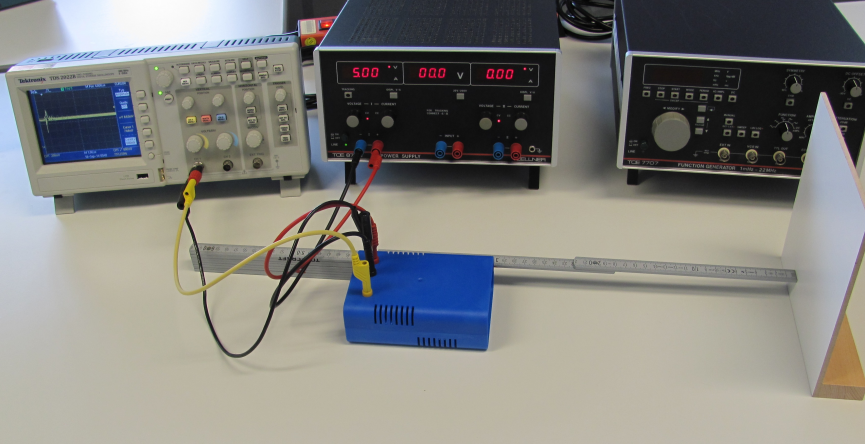
\includegraphics[width=\textwidth]{src/VersuchsAufbauAufg1.png}
	\caption{Aufbau des  Versuchs zur Ermittlung der Kennlinie des Abstandssensors}
	\label{fig:VersuchsAufbauAufg1}
\end{figure}


\section{Messwerte}
\label{chap:VERSUCH_1_MESSWERTE}

In Tabelle \ref{tab:Aufg1Tabelle} sind die eigens abgelesenen Werte sowie die des Oszilloskops abgebildet. Letztere bestehen aus dem Mittelwert von 1500 Spannungswerten und ignorieren dabei den Einschwingvorgang des Sensors.

\begin{table}[H]
\begin{tabular}{|r||r|r|r|r|}
\hline 
 & \multicolumn{2}{r|}{abgelesene Werte} & \multicolumn{2}{r|}{Oszilloskop Werte}\\ 
\hline 
Distanz [cm] & Mittelwert [V] & Delta [mV] & Mittelwert [V] & Delta [mV]\\ 
\hline 
10,0 & 1,5 & 80 & 1,48 & 80 \\ 
\hline 
13,2 & 1,3 & 120 & 1,28 & 80 \\ 
\hline 
16,3 & 1,19 & 100 & 1,17 & 80 \\ 
\hline
19,4 & 1,05 & 32 & 1,03 & 32 \\
\hline
22,6 & 0,949 & 32 & 0,93 & 40 \\
\hline
25,8 & 0,881 & 32 & 0,86 & 24\\
\hline
28,9 & 0,82 & 32 & 0,80 &  32\\
\hline
32,1 & 0,778 & 32 & 0,76 &  32\\
\hline
35,3 & 0,714 & 24 & 0,70 & 32 \\
\hline
38,4 & 0,681 & 64 & 0,67 &  64\\
\hline
41,6 & 0,639 & 88 & 0,63 &  64\\
\hline
44,7  & 0,638 & 80 & 0,63 &  64\\
\hline
47,9  & 0,597 & 80 & 0,59 &  72\\  
\hline
51,1 & 0,581 & 40 & 0,57 &  64\\ 
\hline
54,2 & 0,562 & 56 & 0,55 &  56\\ 
\hline
57,4 & 0,539 & 40 & 0,53 &  56\\ 
\hline
60,5 & 0,503 & 56 & 0,50 &  24\\ 
\hline
63,7 & 0,486 & 40 & 0,48 &  24\\ 
\hline
66,8 & 0,469 & 40 & 0,46 &  32\\ 
\hline
70,0 & 0,453 & 40 & 0,44 &  24\\ 
\hline
\end{tabular} 
\caption{Ergebnisse der abgelesenen Werte und Werte des Oszilloskops }
\label{tab:Aufg1Tabelle}
\end{table}

\section{Auswertung}
\label{chap:VERSUCH_1_AUSWERTUNG}
Im Diagramm (Abbildung \ref{fig:Diagramm1}) ist die Osziloskop Kennlinie durchgehend unterhalb der Linie der abgelesenen Daten.

\begin{figure}[H]
	\centering\small
	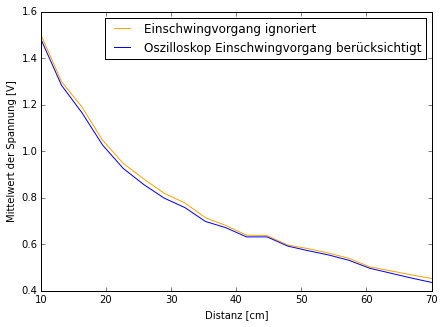
\includegraphics[width=\textwidth]{src/Diagramm1.png}
	\caption{Kennlinie der abgelesenen Werte und der Oszilloskop Werte}
	\label{fig:Diagramm1}
\end{figure}	

\section{Interpretation}
\label{chap:VERSUCH_1_INTERPRETATION}
Die Differenz zwischen Oszilloskop Werten und abgelesenen Werten lässt sich durch den nicht berücksichtigten Einschwingvorgang der ersten 1000 Daten erklären.


%
% CHAPTER Versuch 2
%
\chapter{Versuch 2 - Modellierung der Kennlinie durch lineare Regression}
\label{chap:VERSUCH_2}


\section{Fragestellung, Messprinzip, Aufbau, Messmittel}
\label{chap:VERSUCH_2_FRAGESTELLUNG}

Die Ergebnisse aus Versuch 1 reichen noch nicht aus, um den Sensor als Abstandsmesser verwenden zu können. Deshalb ist eine Umrechnungsvorschrift zu finden, mit der man aus den gemessenen Spannungswerten die dazugehörigen Entfernungswerte berechnen kann.
Diese Übertragungsfunktion wird im folgenden mit Hilfe einer linearen Regression ermittelt.

%[\ref{chap:VERSUCH_1}]

\section{Messwerte}
\label{chap:VERSUCH_2_MESSWERTE}
Die in Versuch 1 ermittelte Kennlinie, sowie Ergebnisse der linearen Regression sind nachfolgend Graphisch dargestellt.
\begin{figure}
\centering\small
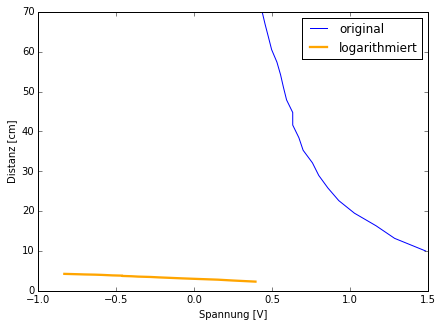
\includegraphics[scale=0.8]{src/Kennlinie2.png}
\caption{Kennlinie vor und nach der Logarithmierung}
\label{fig:KENNLINIE_LOG_ORIG}
\end{figure}
\begin{figure}
\centering\small
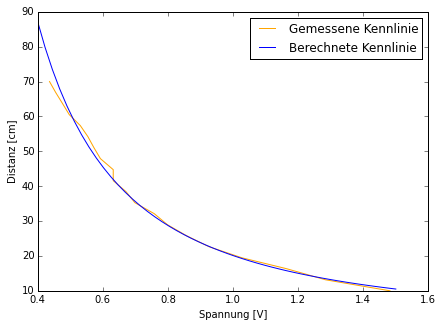
\includegraphics[scale=0.8]{src/Kennlinie1.png}
\caption{Ursprüngliche, gemessene Kennlinie und Kennlinie nach der Regression}
\label{fig:KENNLINIE_FINAL}
\end{figure}

%1.Eingangs und Ausgangswerte logarithmiert
%  lineare Regression
%  Bild Zusammenhang
  
\newpage
\section{Auswertung}
\label{chap:VERSUCH_2_AUSWERTUNG}

%\begin{equation}\label{eq:MATH_FORM}
%T[k]=C-A\cdot\cos\left[\frac{\pi \cdot H_{C}[k-1]}{S}\right]   \mbox{    für } k = %1,2,...,\left(2^{N}-1\right)
%\end{equation}
Da der Sharp-Sensor eine nichtlineare Kennlinie der Form
\begin{equation}\label{eq:NICHT_LIN_KENN}
y=x^a
\end{equation}
 besitzt, müssen die Eingangs- und Ausganswerte zunächst logarithmiert werden. Dadurch entsteht näherungsweise eine Gerade, bei der die lineare Regression verwendet werden kann (Abb.  \ref{fig:KENNLINIE_LOG_ORIG}).
Aus der Regression erhalten wir die Parameter a = -1.6 und b = 3.0 und somit folgende Gerade:
\begin{equation}\label{eq:NICHT_LIN_KENN}
y= -1.6 \cdot x + 3
\end{equation}
Nun muss die vorherige Logarithmierung wieder rückgerechnet werden und wir erhalten die nichtlineare Kennlinie des Sensors wie folgt:
\begin{equation}\label{eq:_KENNLINIE}
y= e^3 \cdot x^{-1.6}
\end{equation}
In der Abbildung \ref{fig:KENNLINIE_FINAL} ist die ursprüngliche Kennlinie vor der Regression, sowie die errechnete Kennlinie nach der Regression zu sehen.
\paragraph{}

%2. logarithmierte Betrachtung y = a+x+b Bild Gerade
%	es müssen keine werte entfernt werden. Messwerte bilden eine Gerade. Keine  	    %extremen Ausreiser auch nicht bei geringen Spannungen bzw. weiter Entfernung
%	y =eb..
%3. Steigung a = -1,6 Schnittpunkt mit Y-Achse b = 3
%  daraus ergibt sich eine Kennlinie wie folgt: y = ...

\section{Interpretation}
\label{chap:VERSUCH_2_INTERPRETATION}

Die gefundene Kennlinie (Abbildung \ref{fig:KENNLINIE_FINAL}) ist in der Form einer abnehmenden Potenzfunktion. Niedrige Spannungswerte entsprechen einem großen Abstand bzw. hohe Spannungswerte einem geringen Abstand, d.h. die Distanz nimmt mit zunehmender Spannung ab. Verschiedene Spannungswerte können nun mit der Übertragungsfunktion in den dazugehörigen Abstand umgerechnet werden.
%interpretation der kennlinie: 
%aus negativen wert des a ergibt sich abnehmender Zusammenhang der Potenzfunktion : Mit %zunehmender Spannung nimmt die Distanz ab




%
% CHAPTER Versuch 3
%
\chapter{Versuch 3 - Flächenmessung mit Fehlerrechnung}
\label{chap:VERSUCH_3}



\section{Fragestellung, Messprinzip, Aufbau, Messmittel}
\label{chap:VERSUCH_3_FRAGESTELLUNG}
Die in Versuch 2 ermittelte Kennlinie ermöglicht nun die Umwandlung von gemessenen Spannungen in Distanzen. Mit Hilfe der Messeinrichtung, bestehend aus Sharp-Sensor Oszilloskop und Kennlinie, ermitteln wir nachfolgend die Breite, Höhe und die Fläche eines Din-A4 Blattes. Dabei wird jeweils der Messfehler mittels des Gaußschen Fehlerfortpflanzungsgesetz berücksichtigt. Die dabei entstehenden Ergebnisse sind danach mit den realen Werten eines Din-A4 Blattes zu vergleichen. Mögliche Abweichungen sind auf eventuelle systematische Fehler in der Kennlinie zu überprüfen.

Messprinzip, Messmittel und Aufbau zur Messung der Distanzen sind wie in Versuch1. (siehe Kapitel \ref{chap:VERSUCH_1_FRAGESTELLUNG}) Zusätzlich wird ein Din-A4 Blatt zur Bestimmung der Distanz verwendet.

\section{Messwerte}
\label{chap:VERSUCH_3_MESSWERTE}
Der Mittelwert der Spannung für Länge und Breite eines Din-A4 Blattes ist in der Tabelle \ref{tab:Aufg3Tabelle} abgebildet. Es sind zum einen abgelesene Werte abgebildet und zum anderen Oszilloskop Werte aus 1500 ermittelten Daten mit Berücksichtigung des Einschwingvorgangs. Nachfolgende Berechnungen beziehen sich auf die Oszilloskop Werte.

\begin{table}[H]
\begin{tabular}{|r||r|r|r|r|}
\hline 
  & abgelesene Werte & Oszilloskop Werte \\ 
\hline 
Distanz [cm] & Mittelwert [V] & Mittelwert [V] \\ 
\hline 
 29,7 & 0,846 & 0,814\\ 
\hline
 21 & 1,02 & 1,004 \\ 
\hline 
\end{tabular} 
\caption{Mittelwert der Spannung jeweils für die Länge und Breite eines Din-A4 Blattes}
\label{tab:Aufg3Tabelle}
\end{table}

\section{Auswertung}
\label{chap:VERSUCH_3_AUSWERTUNG}
\textbf{Breite und Länge}
\paragraph{} Ermittlung des Messfehlers mit Hilfe der Standardabweichung für den Mittelwert $ s_{\bar{x}} $ :
\begin{equation}\label{eq:Standardabw_Mittelwert}
s_{\bar{x}} = \sqrt{\dfrac{1}{n(n-1)}\sum_{i=1}^n(\bar{x}-x_{i})^2}
\end{equation}
Für $ s_{\bar{x}} $ ergibt sich ein Wert von 0.00032. 
Nachfolgend wird von einem Korrekturfaktor $ t = 1,0 $ bei 68\% Sicherheit und $ t = 1,96 $ bei 95\% Sicherheit ausgegangen.
Mit den Mittelwerten aus Tabelle \ref{tab:Aufg3Tabelle} und $ s_{\bar{x}} $ ergibt sich folgende Spannungsmessung mit einem Vertrauensbereich für eine Sicherheit von 68\%:
\begin{equation}\label{eq:Messergebnis68L}
x_{68\%}^{L} = 0,814 \pm \Delta\bar{x}_{68\%}^{L} \enspace [V] \enspace mit \enspace \Delta\bar{x}_{68\%}^{L} = t \cdot s_{\bar{x}} = 0,00032
\end{equation}
\begin{equation}\label{eq:Messergebnis68B}
x_{68\%}^{B} = 1,004 \pm \Delta\bar{x}_{68\%}^{B} \enspace [V] \enspace mit \enspace \Delta\bar{x}_{68\%}^{B} = t \cdot s_{\bar{x}} = 0,00032
\end{equation}
Für eine Sicherheit von 95\%:
\begin{equation}\label{eq:Messergebnis95L}
x_{95\%}^{L} = 0,814 \pm \Delta\bar{x}_{95\%}^{L} \enspace [V]  \enspace mit \enspace \Delta\bar{x}_{95\%}^{L} = t \cdot 2s_{\bar{x}} = 0,0013
\end{equation}
\begin{equation}\label{eq:Messergebnis95B}
x_{95\%}^{B} = 1,004 \pm \Delta\bar{x}_{95\%}^{B} \enspace [V]  \enspace mit \enspace \Delta\bar{x}_{95\%}^{B} = t \cdot 2s_{\bar{x}} = 0,0013
\end{equation}

Mit der Kennlinie (Formel \ref{eq:_KENNLINIE} ) lässt sich mit Hilfe des Gaußschen Fehlerfortpflanzungsgesetzes folgende Formel ableiten:
\begin{equation}\label{eq:GaussFehler}
\Delta y = a \cdot e^{b} \cdot x^{a-1} \cdot \Delta x
\end{equation}
wobei durch einsetzen von $ \Delta\bar{x}_{68\%} $ und $ \Delta\bar{x}_{95\%} $ sich die $\Delta y$ Werte ergeben. Bei Anwendung der Kennlinie (Formel \ref{eq:_KENNLINIE} ) ergibt sich somit eine Länge von 27,97 $\pm$ 0,017 [cm](68\%) bzw. 27,97 $\pm$ 0,069 [cm] (95\%) und eine Breite von 19,98 $\pm$ 0,01 [cm] (68\%) bzw. 19,98 $\pm$ 0,039 [cm](95\%) .

\paragraph{}\textbf{Fläche}
\paragraph{}Zur Berechnung der Fläche wird mit Hilfe des Gaußschen Fehlerfortpflanzungsgesetzes folgende Formel abgeleitet:
\begin{equation}\label{eq:GaussFehler2}
\Delta y =\sqrt{\left(  a \cdot e^{2b} \cdot x_{2}^{a} \cdot x_{1}^{a-1} \cdot \Delta x_{1}\right)^2 + \left(  a \cdot e^{2b} \cdot x_{1}^{a} \cdot x_{2}^{a-1} \cdot \Delta x_{2}\right)^2}
\end{equation}
wobei $x_{1}$ dem Mittelwert der Spannung der Breite und  $x_{2}$ dem Mittelwert der Spannung der Länge entspricht. Somit ergibt sich unter Verwendung der berechneten $\Delta y$ (Formel \ref{eq:Messergebnis68L},
\ref{eq:Messergebnis68B}, \ref{eq:Messergebnis95L}, \ref{eq:Messergebnis95B}) und Multiplikation von Länge und Breite die  Fläche von 558,89 $\pm$ 0,099 [$cm^{2}$](68\%) bzw. 558,89 $\pm$ 1,521 [$cm^{2}$] (95\%).

\section{Interpretation}
\label{chap:VERSUCH_3_INTERPRETATION}
Vergleicht man die erhaltenen Werte der Länge, Breite und Fläche stellt man eine Abweichung von den realen Werten fest.(siehe Tabelle \ref{tab:Aufg3Tabelle2} Zeile 3)

\begin{table}[H]
\begin{tabular}{|r||r|r|r|r|}
\hline 
  & Länge [cm] &  Breite [cm] & Fläche[cm] \\ 
\hline 
 real & 29,7 & 21 & 623,7 \\ 
\hline 
 gemessen & 27,97 & 19,98 & 558,89 \\ 
\hline
$\Delta$ & 1,73 & 1,02 & 64,81 \\ 
\hline 
 angepasst & 29,37 & 21,38 & 627,98 \\ 
\hline
neues $\Delta$ & 0,33 & -0,38 & -4,28 \\ 
\hline 
\end{tabular} 
\caption{Messdifferenzen von Länge, Breite, Fläche}
\label{tab:Aufg3Tabelle2}
\end{table}

Zu erkennen ist eine systematische Unterschätzung der Distanz welche durch Anpassung der Kennlinie um einen konstanten Faktor k = 1,4 aufgehoben werden kann. (siehe Tabelle \ref{tab:Aufg3Tabelle2} Zeile 4,5) 


%
% CHAPTER Anhang
%
\renewcommand\thesection{A.\arabic{section}}
\renewcommand\thesubsection{\thesection.\arabic{subsection}}

\chapter*{Anhang}
\label{chap:APPENDIX}
\addcontentsline{toc}{chapter}{Anhang}
%\setcounter{chapter}{0}
\addtocounter{chapter}{1}
\setcounter{section}{0}

\section{Quellcode}
\label{chap:APPENDIX_SOURCECODE}

\subsection{Quellcode Versuch 1}
\label{chap:APPENDIX_SOURCECODE_V1}

\subsection{Quellcode Versuch 2}
\label{chap:APPENDIX_SOURCECODE_V2}

\subsection{Quellcode Versuch 3}
\label{chap:APPENDIX_SOURCECODE_V3}

\subsection{Quellcode Versuch 4}
\label{chap:APPENDIX_SOURCECODE_V4}


\section{Messergebnisse}
\label{chap:APPENDIX_MEASUREMENT_SOURCE}

%
% Literaturverzeichnis
%
%
% Literaturverzeichnis
%
\phantomsection
\addcontentsline{toc}{chapter}{Literaturverzeichnis}
\bibliography{../references}
\newpage

\end{document}
%------------------------------------
% ╔═╗╔╗╔╔╦╗  ╔╦╗╔═╗╔═╗╦ ╦╔╦╗╔═╗╔╗╔╔╦╗
% ║╣ ║║║ ║║   ║║║ ║║  ║ ║║║║║╣ ║║║ ║ 
% ╚═╝╝╚╝═╩╝  ═╩╝╚═╝╚═╝╚═╝╩ ╩╚═╝╝╚╝ ╩ 
%------------------------------------